\section{Study Protocol and Setup}
\label{sec:StudyProtocol}

%protocol:
\subsection{Conducting Entrance and SRS Surveys}
Prior to their first visit to the lab, the parent was asked to complete the Social Responsiveness Scale (SRS). If the child met the SRS score (minimum of 76 T-score), the same parent would then be asked to complete the entrance survey before their first visit. This same parent was required to accompany the child through all visits.


\subsection{Hand-Washing Trials Protocol Overview}
\label{sec:ProtocolOverview}
The trials were carried out in the washroom inside the HomeLab -- a laboratory specifically designed to emulate the home settings, located on the 12th floor of Toronto Rehab Institute (more details of the experimental environment is described in Section \ref{Sec:ExpSetup}).  Each child would visit the HomeLab once a week with a total of six visits with his/her parent. The six visits would consist of three kinds of phases. The three phases are namely the baseline phase (Phase A) and the intervention phases (Phase B and Phase C). In Phase A, the child would be asked to wash hands by him/herself as independently as possible. The parent was instructed to provide assistance to the child as the parent saw necessary.  In Phase B, the child would be assisted by the robot NAO alone.  The parent was out of view in the room adjacent to the washroom, and came into the washroom to guide the child to continue if the child got stuck or finished early and was leaving the washroom.  In Phase C, the child would be assisted by NAO and the parent together.  The parent remained in the washroom and assisted robot NAO in its prompts.  The parent is left to his/her best judgment in how to work best together with the robot.

Each visit would take about an hour to an hour and a half. The child was asked to wash his/her hands eight times for every visit, for a total of forty-eight trials per child.  This way, the consecutive trials conducted within a day would hopefully be not too much for the child to cause fatigue.  The child and his/her parent could take short breaks after each hand-washing trial.  The break could last as long as the child needed until he/she was willing to continue the trial. If the parent felt the need, they could leave and come back to finish the rest of the day's trials another day. They would not be withdrawn from the study unless requested.

We would conduct the phases in the order A-A-B-C-C-B (i.e. parent alone phase - robot alone phase - robot parent phase - 2nd robot alone phase).  By splitting phase B to flank phase C, we can compare first Phase B and second Phase B to see how much did learning in Phase C affect our results.  We aimed to approximately have sixteen trials per phase, which gives a good sample size for both quantitative and qualitative analyses.  This means first phase B and second phase B would have about eight trials each.  Note that the number of trials for each phase might be adjusted as by the researcher depending on the ongoing data analysis, and the interview would be used as a basis for such adjustment.  More detail is discussed in Section \ref{sec:ConductingInterviews} - Conducting Interviews and the Basis of Sample Selection.


\subsection{Experiment Setup}
\label{Sec:ExpSetup}
The equipment was set up near the sink, which included a NAO robot, an overhead camera, a scene camera, and a Kinect camera. The NAO robot is a small half-torso humanoid robot and was screw-mounted on the sink countertop at the top left corner (please see Figure \ref{fig:ExpSetup}). The NAO robot delivered verbal and gesture prompts to the children with ASD while they were performing the hand-washing tasks.  The overhead camera was installed on the wall/mirror right above the sink. The overhead camera recorded objects on the sink countertop (e.g., taps, faucet, soap, and towel). The purpose of the overhead camera was to capture the hand actions of the child during hand-washing in order to track the child's progress along the tasks. The scene camera was placed on the floor on a camera stand with its field of view including all objects in the scene (e.g., robot, child, and objects on sink countertop). The purpose of the scene camera was to capture the child's engagement and attention during the prompts as well as during task executions. The Kinect camera was mounted on the sink countertop underneath the mirror and behind the tap. The Kinect camera recorded mainly the child's face. The purpose of the Kinect camera was to capture the child's face during hand-washing for the development of an automatic algorithm that estimates the child's gaze direction in real-time. Examples of the images captured by the three cameras are shown in Figure \ref{fig:CameraViews}.
\begin{figure}[H]
	\centering
	\begin{subfigure}[b]{0.49\textwidth}
		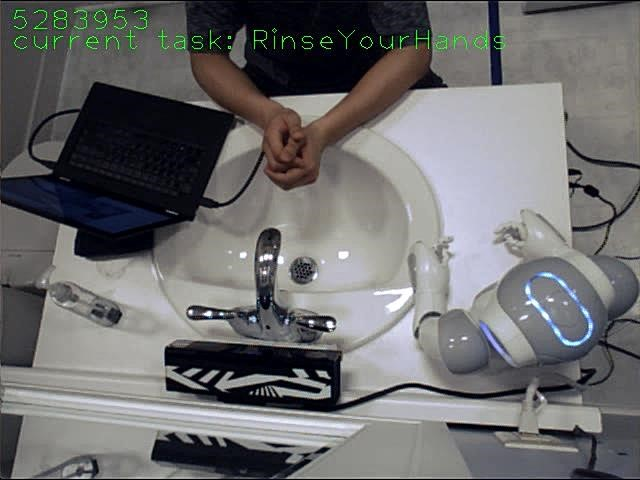
\includegraphics[width=1.1\linewidth]{./img/overhead_view.jpg}
		\caption{Overhead Camera View}
%		\label{fig:7TotalNumberofIncompleteSteps-BeforeParentorRobotPrompts}
	\end{subfigure}
	
	
	\begin{subfigure}[b]{0.49\textwidth}
		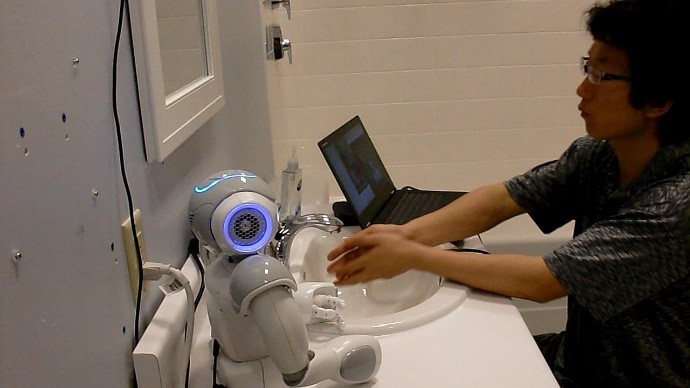
\includegraphics[width=1.1\linewidth]{./img/scene_view.jpg}
		\caption{Scene Camera View}
%		\label{fig:6TotalNumberofIncompleteSteps-BeforeParentPrompts}
	\end{subfigure}%
	
	
	\begin{subfigure}[b]{0.49\textwidth}
		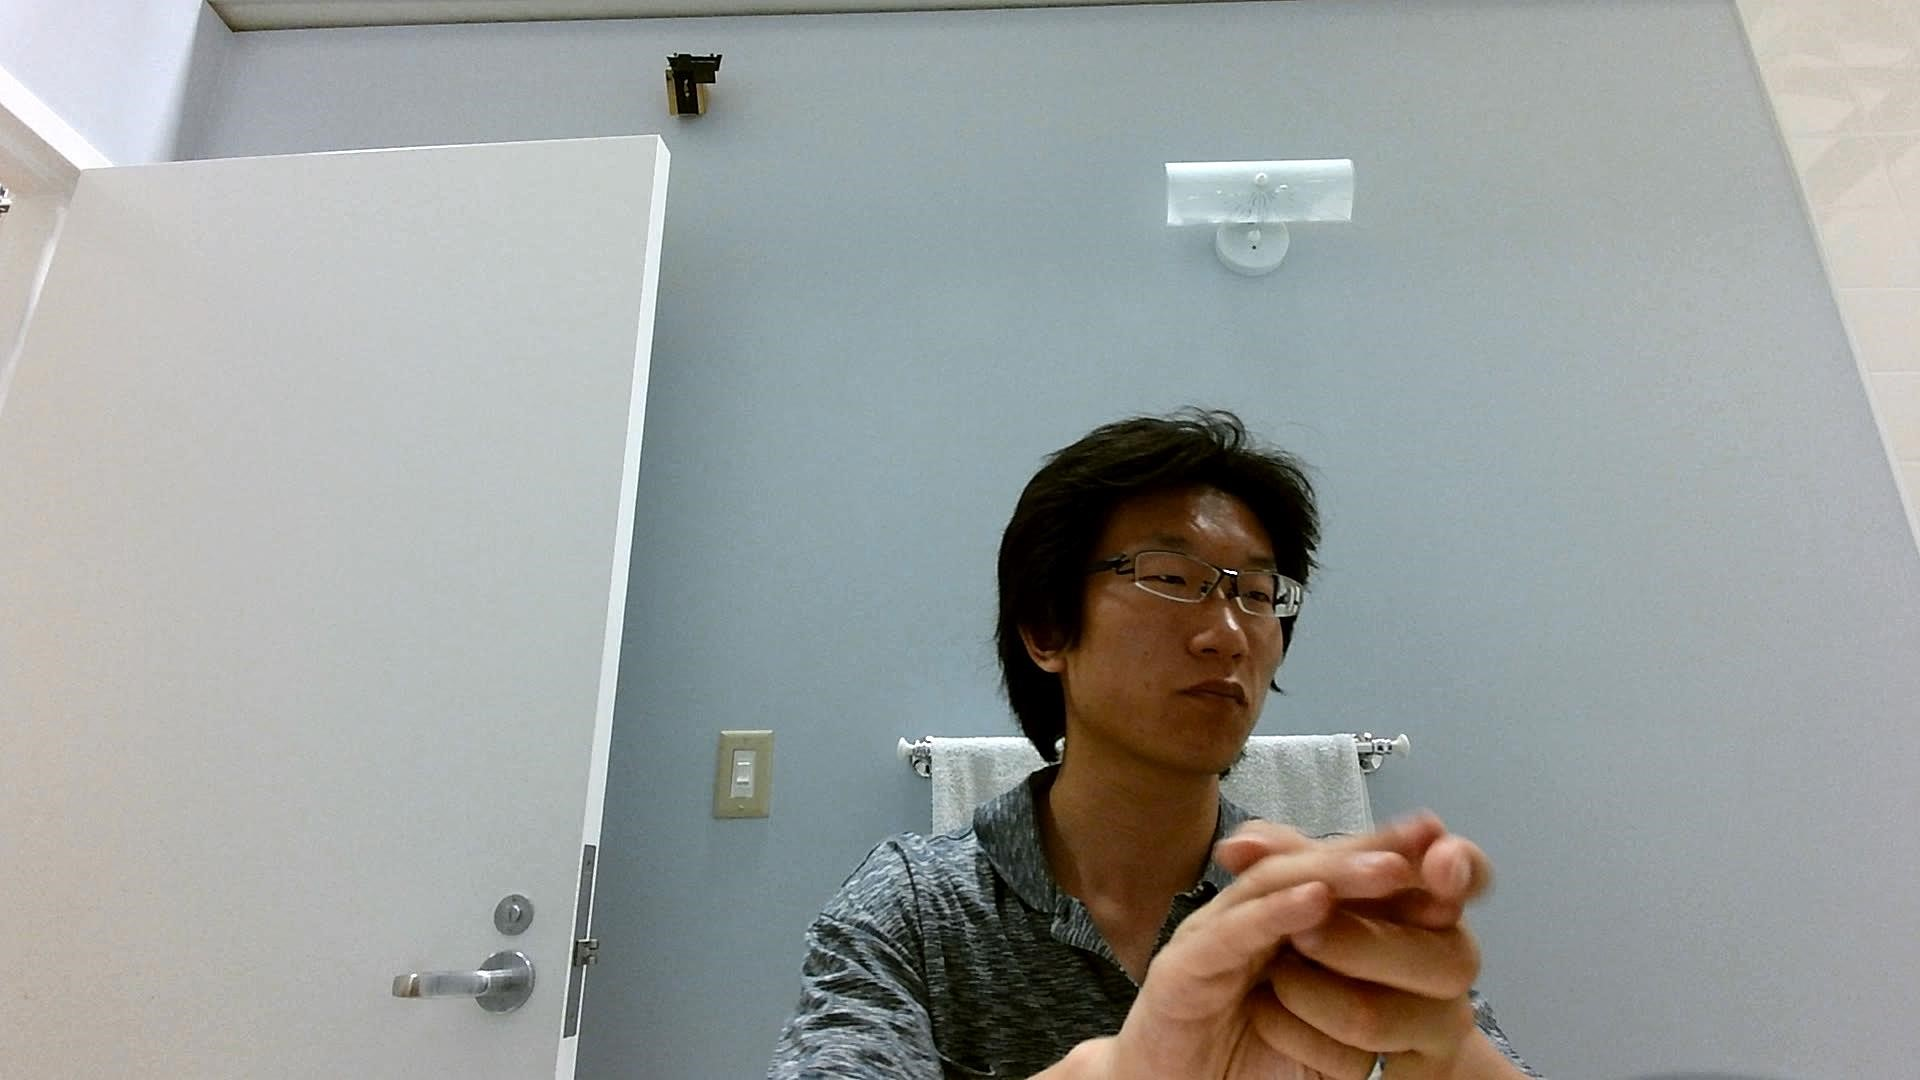
\includegraphics[width=1.1\linewidth]{./img/kinect_view}
		\caption{Kinect Camera View}
%		\label{fig:5TotalNumberofIncompleteSteps-BeforePhyiscalPrompts}
	\end{subfigure}%
	
	\caption{The views of the three cameras used in the WoZ study.}
	\label{fig:CameraViews}
\end{figure}


A touchscreen laptop was used during the study by the student researcher to control the robot and the virtual avatar displayed on the LCD screen. It connected to the robot wirelessly. The laptop also connected to the overhead and Kinect cameras through USB cables to provide real-time video feed. The data collected from the cameras was saved temporarily in the laptop hard-drive.

\subsection{Specific Protocol}
\label{sec:SpecificProtocol}
The hand-washing activity was broken down into seven steps: turn on the water, wet your hands, get some soap, scrub your hands, rinse your hands, turn off the water, and dry your hands.  These steps were modified based on Bimbrahw et al.'s pilot study \cite{bimbrahw2012investigating}. These constituted the same steps as Bimbrahw's except that the first (i.e. turn on the water and wet your hands) and the last step (i.e. turn off the water and dry your hands) are now four individual steps to ensure that each step only involved one action.

\paragraph{Phase A (Baseline Phase)}
In the baseline phase, the child would be asked to complete the hand-washing as independently as possible. During this phase, the parent would be present in the washroom while the child was completing the hand-washing steps. The parent would verbally prompt and/or physically assist the child and give positive reinforcements to the child whenever the parent feels necessary.  Minimal restrictions or guidances were presented to the parent by the researcher, so that what the parent thought were important could become apparent to the researcher.

\paragraph{Phases B and C (Intervention Phases)}
In the intervention phases, the child would be asked to wash his/her hands with the help of NAO or of both NAO and the parent in the washroom. During every trial, NAO and/or the parent would wait for the child to start each step. If the child experienced troubles, an appropriate prompt would be delivered from NAO in order to help the child complete the step. If the child did not respond to NAO's prompt, an attention grabber would be delivered to capture the child's attention to the prompting agent. The attention grabber could be repeated for a second time if the child failed to respond to the first one.  After successfully grabbing the child's attention, the prompt would be repeated.  A verbal reward would be delivered to the child when he/she completed a step.

The parent's role in phase B and C differs in that, in phase C, the parent would take a more active role to prompt the child of what to do by standing next to the child.  On the other hand, in phase B, the parent would be out of view and coming in to prompt only when the robot is unable to continue, and for the purpose of reminding the child to listen to the robot, but leaving the prompting of the specifics of the steps to the robot.  Of course, for both phases, if the child didn't respond to any of the prompts, the parent would need to physically intervene and complete the step together, similar to phase A.  After the physical intervention in phase B, the parent would then instruct and encourage the child to continue the rest of the hand-washing steps on his/her own by following the robot.  Both phase B and C are important.  Phase B serves to test if NAO can independently assist the child through hand-washing with minimal parent involvement.  Phase C serves to investigate whether and why would NAO be more effective in assisting the child when parent is present.  Comparing phase B and C would potentially yield areas of improvements for NAO.

There are three prompt categories that the NAO robot would deliver when interacting with the child (please see Table \ref{tab:RobotPrompts} for the specifics of each prompt used):
\begin{enumerate}
	\item \textbf{Step Prompt} (to prompt the child through a hand-washing step):
	
	A verbal prompt is delivered, such as “Please [step name]” (e.g. “Please turn on the water.”).  Synchronous to the verbal, a visual prompt is also be delivered. This is a two-part gesture prompt of: first, demonstrating the motion of interaction while looking at the child (i.e. MoDemo); second, pointing to the sink object (e.g. the tap) while looking at the object (i.e. ObjPt). A maximum of two prompts is given to the child. If the child does not respond to the second prompt or has started the step but does not complete the step within the a reasonable time, the parent is asked to help the child complete the step. 
	
	\item \textbf{Attention Grabber} (to capture the child's attention to the NAO robot): 
	
	A verbal prompt is delivered, such as “Hi, [child's name]!”  Synchronous to the verbal, a visual prompt is also delivered. This is an attention grabbing gesture of waving and looking at the child (i.e. AG). A maximum of two attention grabbers is given to the child in order to get his/her attention to look at the robot.  The parent is asked to instruct the child to look at the robot if he/she does not respond to the second attention grabber. 
	
	\item \textbf{Reward} (to provide positive reinforcement when the child attempts a step without the help from his/her parent): 
	
	A verbal reward (i.e. “Great!”) is delivered while looking at the child and switching back and forth the colors of the light-emitting diodes (LEDs) on the eyes after successfully performing a step (i.e. REW).
\end{enumerate}
\begin{table}[h]
	\centering
	\begin{tabular}{ |l| p{4cm} | p{8cm} | }
		\hline
			&	\textbf{Verbal Prompt}	&	\textbf{Robot Gestures}	\\	\hline
			
		\textbf{Attention Grabber}	&	Hi, [child's name]!	&	Waving and looking at the child.	\\	\hline
		
		\multirow{7}{*}{\textbf{Task Prompts}}	&	Turn on the water!	&	Turning right wrist clockwise while looking at the child, then pointing and looking at the tap.	\\	\cline{2-3}
		&	Wet your hands.	&	Holding out hands while looking at the child, then pointing and looking at the running water.	\\	\cline{2-3}
		&	Get some soap.	&	Pressing down right hand with left hand collecting from below while looking at the child, then pointing and looking at the soap.	\\	\cline{2-3}
		&	Scrub your hands.	&	Scrubbing both hands while looking at the child, then pointing and looking at the child's hands.	\\	\cline{2-3}
		&	Rinse your hands.	&	Holding out hands while looking at the child, then pointing and looking at the running water.	\\	\cline{2-3}
		&	Turn off the water.	&	Turning right wrist counterclockwise while looking at the child, then pointing and looking at the tap.	\\	\cline{2-3}
		&	Dry your hands.	&	Wiping one hand against the other while looking at the child, then pointing and looking at the towel.	\\	\hline
		
		\textbf{Reward}	&	Great!	&	No gestures. Flashing multicolor LEDs on the eyes while looking at the child.	\\	\hline
		
		\textbf{Intro}	&	Hi, [child's name]! Let's start washing hands.	&	Giving an attention grabber gesture followed by a simple conversational gesture while looking at the child.	\\	\hline
		
		\textbf{Re-intro}	&	Let's continue washing hands.	&	Giving a simple conversational gesture while looking at the child.	\\	\hline
		
		\textbf{Outro}	&	Good job, [child's name]! You are all done.	&	Fist pumping in the air, followed by an all done gesture. Flashing multicolor LEDs on the eyes while looking at the child.	\\	\hline
	\end{tabular}
\caption{The Robot Prompts -- Detailed Descriptions.}
\label{tab:RobotPrompts}
\end{table}

For each trial, in addition to the three prompt categories stated above, the NAO robot would also deliver a short introduction before the start of each trial, a re-intro after the parent finished assisting the child through a step, and an outro at the end of each trial. The introduction is a two-part prompt. The first part is an attention grabber. The second part consists of a verbal prompt (i.e. “Let's start washing hands.”) with a simple conversational gesture. The re-intro is a verbal prompt (i.e. “Let's continue washing hands.”) with a simple conversational gesture. Same as the introduction, the outro is a two-part prompt. The first part consists of a verbal prompt (i.e. “Good job, [child's name]!”) with a gesture of fist pumping in the air. The second part consists of a verbal prompt (i.e. “You are all done.”) with a gesture signifying all the hand-washing steps have been done.

\subsection{Conducting Interviews and the Basis of Sample Selection}
\label{sec:ConductingInterviews}
The interview with the parent would be conducted by the researcher during every break between trials.  This is to discuss what happened in the last trial, why the child behaved this way, whether we need to change the robot prompts for improving effectiveness, whether to change the protocol to focus on certain aspects of the study more, and how many more trials of the current phase should we do.  Also, the researcher might also request certain ways the parent was to assist and guide the child, so to explore the influence of the parent on child's interaction with the robot.  Although conducted in an informal conversation format, this interviewing, discussion, and reflection process is a form of qualitative analysis similar to that of making observational field notes.  Thus, the results of these discussions were then used as basis for sample selection, revising the robot behavior and study protocol for the next trials.  This process was continued iteratively, which models after the theoretical sampling method defined in Section \ref{sec:CaseSelectionAndSampleSelection}.  And within the theoretical sampling approach, we adopted the maximum variation sampling method by varying the degree of the parent's involvement.

\subsection{Conducting Post-intervention Surveys}
During the last visit, the same parent who completed the entrance survey would be asked to fill out the post-intervention survey.

\subsection{Data Collection}
All trials were video recorded by the overhead, the scene, and the Kinect cameras and audio recorded by the microphone from the scene camera.  The overhead and scene video data would be reviewed and annotated by an annotator. The overhead video data would be used to score the participants' prompt compliance and hand-washing performance. The scene video data would be used to evaluate the participants' engagement during the whole activity. Possible areas of improvement of robot prompting will be explored, based on its observed effects on engagement, compliance, and performance.

The Kinect video data would not be annotated. Instead, it would be used to evaluate the automatic gaze estimation algorithm that we would develop. Specifically, the Kinect video data would be used by the gaze estimation algorithm as input and the outputted predictions would be compared with annotations of the scene video data to evaluate the algorithm's prediction accuracy.



\subsection{Ethics}
The WoZ pilot study was approved by the Research Ethics Board (REB) of University Health Network (UHN), belonging to which is the Toronto Rehab Hospital, where the study was conducted.

\paragraph{Consent and Assent}
Participants were given a package of consent/assent forms prior to starting the study. One of the parents would need to provide their consent for their child and themselves to participate in the study. In addition, child participants would need to provide their assent to participate in their every visit of the study. 

Interested families would receive an information/consent package prior to starting of the study. This package includes consent/assent forms for participation in the study for the parent and child with ASD (these forms include study details and research contact information) as well as consent to be videotaped for the parent and child with ASD. Consent from the parent and assent from the child with ASD would be given if and when they feel comfortable that they understand the information presented. Potential participants of both parents and children had up to a week to decide if they would like to participate, although they may consent to participate as soon as they feel comfortable doing so. Parents would need to provide their consent for their children and themselves to participate in the study. In addition, child participants would need to provide their assent in their every visit of the HomeLab during the study to participate. Parents would be required to consent to having their children and themselves videotaped during the study. The parents would be informed that they and their children may withdraw from the study at any time without penalty.

\paragraph{Confidentiality}
Each participating family (parent and child with ASD pair) would be assigned a code number when they sign the consent/assent. All data in the study would be labelled with these code numbers only - the names of the participants would appear only on the information and consent/assent forms and would be kept confidential. Consent forms would be placed in a secure and locked area in the PI's laboratory, with access exclusively restricted to the research team. All forms will be destroyed seven years after the study publication. 

The information and data collected would remain strictly confidential and would not affect any of the participants (both the parent and the child)' employment, care, or treatment in any way. A code number would be assigned to each parent and child participant when they give consent. This code number, instead of their name, were used for all data collection and analysis. Direct quotes may be included in the final research paper but names would not be used in any report or publication. Privacy of participants (both the parents and the children) were ensured by omitting all participant information from participant data, by employing data encryption, and by storing data on a secure server.  If and only if participants consent, participants (both the parents and the children) video data could be presented for educational purposes.  If any images or videos were used in presentations and publications, faces and other identifiable features would be masked.

Both the video and audio data would be stored temporarily on the touchscreen laptop's hard drive during each child's visit. The data would be encrypted and transferred to the TRI servers as soon as after each child's visit. The portable devices, such as USB sticks, would be used to transfer the data to the TRI servers. All files stored in the portable devices would be password protected and encrypted. The data on the laptop's hard drive and the portable devices would then be purged immediately after transfer. 

\paragraph{Data Storage}
All soft (electronic) data would be encrypted before any transfer is made. All data would be password protected and be stored on the TRI servers with access restricted to the research team. The laptop used for the study were password protected so that only the research team has the access to it. All computerized data would be password protected. All survey data would be stored in a locked cabinet different from where the consent forms are stored. Access to all the data would be restricted only to the supervisor and researchers involved in the project. 

After the study is completed and the results of the study are published, data will be stored for at least seven years from study closure. All data will be destroyed seven years after the study closure. Data contained on paper material will be destroyed by shredding the material. Data contained on electronic media will be destroyed by erasing or other removing the data in such a way that it cannot be retrieved. 

